\title{CMPS 240 Artificial Intelligence\\RPS-Safari}
\author{Kerui Huang\\khuang7@ucsc.edu}
\date{\today}
\documentclass[10pt]{article}
\usepackage[cm]{fullpage}
\usepackage{graphicx}
\usepackage{wrapfig}
\usepackage{bm}
\usepackage{amssymb}
\usepackage{amsmath}
\usepackage{epsfig}
\begin{document}
\maketitle

\section{INTRODUCTION}
Rock-paper-scissors (RPS) is a simple game, but it does involve some fundamental problems about the fields of artificial intelligence, such as how to design a decent algorithm to make the computation more intelligent.

Theoretically, if someone is playing RPS completely randomly, it is impossible to gain any advantage against this player. However, human players tend not to be completely random, neither do most machines. Therefore,we are interested in finding a computational method, or say an algorithm, to make an agent computational ``intelligent".

In this project, we are supposed to design an intelligent agent to play RPS with other agents. Initially, each agent has 1 point at the beginning and then join the tournament. For each tournament, agents play against each other over 1000 rounds. The final results depend on the performance of the agent in each round. For each round, the score of an agent is updated by 
$$bet * sign(\#victims(x)-\#killers(x)) - sign(bet)* *total-returns*$$
$*total-returns*$ is a global variable provided by the environment and each of its entries maintains the information about R, P or S respectively. 

For example, if the total return of R (the first entry) is 3. In the current round, there are 4 Rocks, 5 Papers and 6 Scissors, then the total return of R will be updated as: $*total-returns*(R) = 3 + sign(\# victim(R) - \# killer(R)) = 3 + sign(6 - 5) = 4$. Therefore, it means for each round the total past return of the play an agent makes, times the sign of the bet size, will be subtracted from his score.

Furthermore, we have another global variable named $*avg-returns*$ to use, which maintains the average number of total R, P, S and the average score of each agent. This variable is updated after each round and is reset per tournament.

In addition, we are allowed to use three semi-local variables to do whatever we want. This is useful, because it enables us to store some past information which can help our agents make a decision based on the previous performance.

Finally, the source file of the agent is up to 150 80-character lines of code.

\section{STRATEGY}
\subsection{Why Not Random}
Playing randomly is somehow a good strategy. Because it is random, there is no pattern under the hood to be discovered. At this point, it can successfully confuse opponents. 

However, it also means that it is closed, namely, it does not learn. What if an opponent always plays rock? If the agent perceives it, it can always play paper to beat this opponent. This strategy is apparently better than playing randomly in this case. Actually, as mentioned above, players are usually non-random. In this sense, maybe we can use heuristic algorithms to build a strong agent which is likely to predict others' behavior.

\subsection{My Strategy}

\subsubsection{Choice}
First, the agent should know which one to play. Rock, paper or scissor? Note that we have five inputs -- history, scores, my score, *avg-returns* and *total-returns*. We can gain detailed information about how many times R, P, S appears in each round through history and have a very basic sense of it by simply looking at *avg-returns*. Besides, we can also perceive the performance of each agent through scores and *avg-returns*. However, it is not enough to know which one, R, P or S, is the best choice, because we don't know how well each choice performed in the past. Fortunately, *total-returns* provides some guidance, because it reveals the performance of each choice so far. Based on the number of his victims and killers, a choice may win or lose. If a choice wins, its corresponding entry in *total-return* will be updated by +1, while if it loses, the entry will be updated by -1. That is why it somehow reflects the performance of each choice. Thus, we use this variable to help us make a decision.

However, things are not that easy. We should also keep in mind how our scores are updated. The term $- sign(bet)* *total-returns*$ introduces chaos and unpredictable patterns, which makes the work complicated and harder. Thus, we should be constantly gauge the risk and reward, and try to find the optimum bet and the optimum one to bet on. After some experiments, the interesting phenomenon I observed is that this term seems to have more significant influence on the results than it is positive impact discussed above does. Namely, even though a choice with a high value in *total-returns* seems to be a winner, we should avoid betting on it, because we will lose a lot of scores as long as our guess is wrong. The empirical experiments shows conservative strategy is better than aggressive strategy. Therefore, the strategy is very straightforward here. We can simply search for the minimum value of *total-returns* and then choose the corresponding choice as our own choice. Here is the example:
\begin{quote}
\textbf{Example 1:}\\
Suppose $*total-returns*=(4\ 3\ 5)$, then we are more likely to play P, which has the lowest entry in *total-returns*.
\end{quote}


\subsubsection{Weight}
The second question is how much the agent bets for this round. After\footnote{Again, for the first round, the agent just randomly weighs its bet. In addition, the bet surely cannot break  our RPS-Safari rules. Please see the basic requirements on the website.} the first round, the agent knows how it performed in the last round. So here, the idea is to better the weight of its bet according to its past performance. My assumption is:
\begin{quote}
\textbf{Assumption 1:} \textit{If the agent played really well in previous rounds, it makes sense that it should be more confident of itself and then bet more than last round, or vice versa.}
\end{quote}

Besides this reasonable assumption, some other scenarios should be considered. For example, as Prof. Levinson mentioned in the lecture, even though an agent wins every time, it is not a good idea to bet all it has. Once it loses, it loses all. Therefore, my considerations are:
\begin{quote}
\begin{itemize}
\item \textbf{Case 1:} When an agent plays very well gains a very high score, it is good to be more conservative, because the important thing is to keep its upper hand. ``Conservative" means it almost keeps its old weight, not increases it dramatically any more.
\item \textbf{Case 2:} When an agent plays somewhat well and gains a slightly high score and it keeps performing very well, since it has not reached a very high score, it is advisable to let it be more aggressive and consequently add more weight to its bet in order to make improvements faster.
\item \textbf{Case 3:} When an agent just starts its adventure or it played so far neither too bad nor very well, it had better be conservative and wait until it gains more experience after rounds. When it performs better and better (Case 2), it can begin to bet more.
\item \textbf{Case 4:} So far, I only discussed about the scenarios in which an agent plays not bad. What if the agent plays very bad? If an agent plays bad, it sort of means that it cannot trust itself. However, it is still helpful, because it can just take the opposite decision. So, bad cases become simple -- the agent just reverses its original choice (which is made based on the first three cases).
\end{itemize}
\end{quote}

However, the cases above are only concerned about the current performance compared with the very initial state, which does not give us the whole picture. For example, an agent may play very well and gain a very high score after a few rounds. However, it recently did not play very well, and began to lose points. If we only measure the difference between its initial score and current score, we may lose our sense of trend. Trend is very significant since it tells what will probably happen in the future. Therefore, we would like to have some other scenarios:
\begin{quote}
\begin{itemize}
\item \textbf{Case 5:} When an agent keeps playing well recently, even though its score is not very high, we are still willing to let it bet more.
\item \textbf{Case 6:} When an agent keeps playing bad recently, even though its score is very high, we may not trust it like before and let it bet less.
\end{itemize}
\end{quote}

In this way, we can see that both current performance and past performance are taken into consideration. The next question is to decide their proportions. We can use a variable $w$ to tune the weight of them.
$$
x = w\times past\ performance + (1-w)\times current\ performance
$$
The variable $x$ is the parameter I use for the final calculating of bet weight, which follows the cases 1- 4.

The current performance is straightforward. We can just use the difference between its current score and initial score as the current performance, which is:
$$
current\ performance = current\ score - 1
$$

We can compute past performance by using a semi-local variable. Here, I use a semi-local variable to store the sequence of my own score. To calculate the past performance, I weigh each difference between two scores differently, based on time.

\begin{quote}
\textbf{Example 2:}\\
Suppose my scores are (-1 -3 -4 -5 0 1 2) \footnote{The leftmost value is the most recent score.}, then I the differences are: D = (2 1 1 -5 -1 -1). It is obvious that the agent recently performed well while it used to performed bad. We weigh its recent performance more. Therefore, we may calculate the past performance as:
$$
past\ performance = \sum_{i=1}^{6}(7-i)*D_i = 6*2 +5*1 + 4*1 + 3*(-5) + 2*(-1) + 1*(-1) = 3
$$
\end{quote}
The result is positive, which means the agent is considered to play well in the past. However, its current performance, which is $-1 - 1 = -2$, indicates that its performance so far is not very good. Therefore, we cannot believe it that much only because it is performing well now. Its past bad performance is supposed to have bad influence on the weight of its decision. That is why we consider both its past performance and current performance when we calculate $x$, the variable we use for calculating the final size of bet as below:

$$
weight=ceiling(f(x))
$$
$$
f(x)=10\times arctan(.05\times (x - 100)) + 14, when\ score\geq 0
$$

The term 10 controls the scale of the weight, since the original $arctan$ function is too small to fit our score scale. The term .05 controls how fast the agent increase the weight of its play. The term 100 means the point at which the agent thinks it should make the fastest improvement. Namely, when the agent reaches 100 points, the increment of the weight is largest.

The term 14 is used for bounding the absolute value of the weight. Because 
$$
\lim_{x \to -\infty} (10\times arctan(.05\times (x - 100))) = -15.708
$$ and we need to make sure the bet is positive \footnote{Here we consider positive cases only. For negative cases, we will simply change the sign later.}, we need to add 14 to ensure it is positive when score is 0.

Figure \ref{figure:a} shows the change of the weight for positive cases.

\begin{figure}
\centering
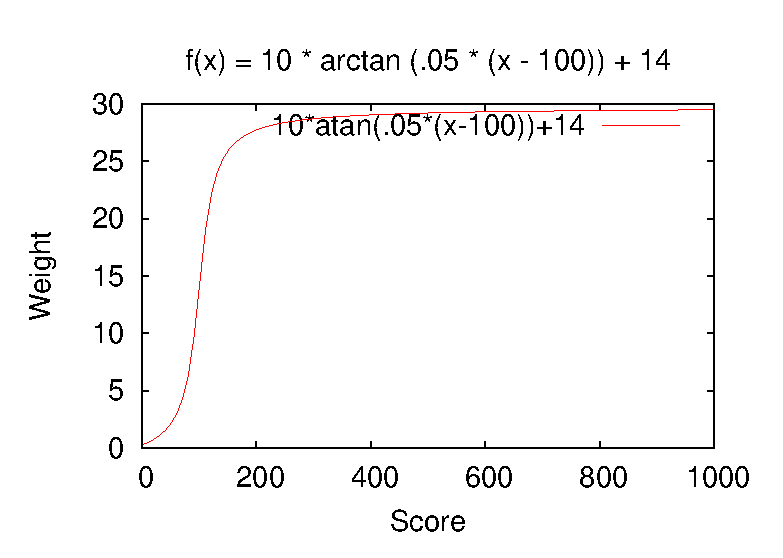
\epsfig{file=b.eps, height=2in, width=2.5in}
\caption{The function $f(x)=10\times arctan(.05\times (x - 100)) + 14, when\ score\geq 0$}
\label{figure:a}
\end{figure}

\section{EXPERIMENTS}
I ran tournament 10 times. The results show that my P3 agent obviously performed much better than my P2 agent. Table \ref{tab:res1} shows the scores of my two agents after each tournament. Table \ref{tab:res2} shows their corresponding ranks.

\begin{table}
\caption{Experiment results of scores for each tournament}
\label{tab:res1}
\center
\begin{tabular}{ c c c c c c c c c c c } \hline
Agent		&1		&2		&3		&4		&5		&6		&7		&8		&9		&10\\ \hline
KHUANG7		&35.0	&28.4	&35.0	&30.2	&31.4	&30.8	&30.2	&29.6	&30.2	&30.2 \\
KHUANG7-P3	&13.3	&22.9	&20.5	&25.3	&26.6	&25.9	&24.7	&25.3	&27.2	&24.1 \\ \hline
\end{tabular}
\end{table}

\begin{table}
\caption{Experiment results of ranks for each tournament}
\label{tab:res2}
\center
\begin{tabular}{ c c c c c c c c c c c } \hline
Agent		&1		&2		&3		&4		&5		&6		&7		&8		&9		&10\\ \hline
KHUANG7		&1		&14		&1		&9		&8		&9		&9		&10		&9		&9\\
KHUANG7-P3	&39		&25		&27		&24		&18		&19		&20		&20		&16		&21\\ \hline
\end{tabular}
\end{table}

%\begin{table}
%\caption{Comparing early result rates.($c=\frac{|A||B|M}{(|A|+|B|)^2FT}$)}
%\label{tab:rrcomp}
%\center
%\begin{tabular}{|c|c|} \hline
%& $F=1.2, T_{ri}=T_{wt}=T_{rt}=T$ \\ \hline
%Symmetric Hash & $c$ (Must fit in memory)\\ \hline
%Hash Ripple & $ 0.5c $ \\ \hline
%SMS-Join & $ 0.6c $ \\ \hline
%Block Ripple & $ \frac{2k+1}{k+2}c:c, 1.25c, 1.40c, ... $ \\ \hline
%PR-Join ($ \gamma=1 $) & $ c, 1.7c, 3.2c, 6.2c, 12.2c, ... $ \\ \hline
%\end{tabular}
%\end{table}

%\begin{figure}
%\centering
%\includegraphics[width=50mm]{size.jpeg}
%\caption{A 10G relation joins a 20G relation}
%\label{figure:size}
%\end{figure}
%\bibliographystyle{abbrv}
%\bibliography{bib}
\end{document} 
